\part{Methods}
\label{part:methods}

\chapter{Simulations}

The system studied in this thesis consists of an ensemble of paramagnetic colloidal particles confined in a quasi-two-dimensional geometry and subjected to an externally applied precessing conic magnetic field. Each colloid is a spherical particle of radius $r_{\mathrm{mag}}$ suspended in a Newtonian fluid of dynamic viscosity $\eta$. The suspension is bounded by two parallel glass plates separated by a distance $h$, such that $h \lesssim 2R$. This strong confinement restricts particle motion primarily to two dimensions, while still allowing limited vertical displacement. 

\begin{figure}
  \begin{center}
    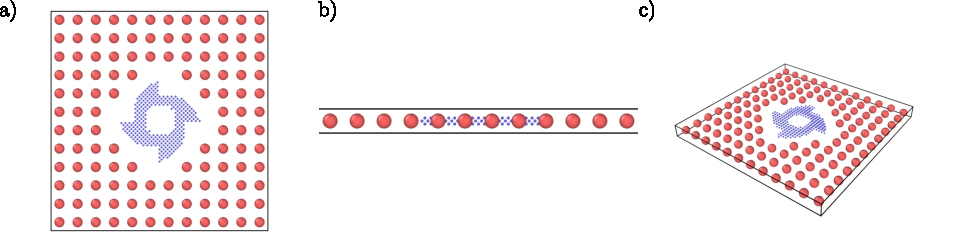
\includegraphics[width=0.95\textwidth]{figures/system.pdf}
  \end{center}
  \caption[System overview.]{System overview for a spin up ratchet}\label{fig:system}
\end{figure}


Numerical simulations provide a powerful framework to reproduce and analyze physical phenomena under controlled conditions. Unlike experiments, they allow for precise manipulation of initial parameters, systematic testing of hypotheses, and straightforward replication of results. In particular, simulations are invaluable when dealing with microscopic systems, where stochastic effects and complex interactions can make experimental observations challenging. 

In this thesis, numerical simulations are employed to study the dynamics of colloidal systems at the microscale. Such systems are often dominated by thermal fluctuations and many-body interactions, making them difficult to probe experimentally without advanced imaging and data analysis techniques. The primary computational approach used here is \textit{molecular dynamics} (MD), which will be described in detail in the following sections. MD enables the integration of particle trajectories under the influence of deterministic and stochastic forces, providing direct access to observables such as mean-squared displacements, velocity correlations, and transport coefficients.

\section{Molecular dynamics}



This thesis explores the physics of the system by using molecular dynamics, where randomness enters through thermal noise. As we saw in \ref{stochasticrepresentation}, the interactions can be derived from classical mechanics. In this case, Newton’s second law gives the starting point to calculate the forces acting on a single particle. In other words, at each iteration of the simulation we need to evaluate the forces that each particle experiences. Taking equation~(\ref{eq:newton}) as a starting point, and adding labels for the different interactions, we obtain:

\begin{equation}
  m_i\ddot{\vec{x_i}} = F^{collision}_i + F^{drag}_i + \eta(t)\text{,}
  \label{eq:langevinratchet}
\end{equation}

where $m_i$ is the mass of particle $i$, $\vec{x_i}$ its position, and $F^{drag}_i$ is the viscous force, written as $-\lambda \dot{\vec{x}}_i$, with $\lambda$ the drag coefficient of the fluid. Since we are working at a scale where inertial effects are negligible, the term $m_i\ddot{\vec{x_i}}$ can be dropped. The random force $\eta(t)$ represents collisions with the solvent particles. In this thesis, $\eta$ is taken as a Gaussian random force with $\expval{\eta} = 0$ and correlation $\expval{\eta_i(t)\eta_j(t')} = 2k_B T \lambda \delta_{i,j}\delta(t-t')$. This form will be used for non-paramagnetic particles.

For paramagnetic particles, we need to add the contribution of dipole–dipole interactions, which gives the modified equation:

\begin{equation}
  m_i\ddot{\vec{x_i}} = F^{collision}_i + F^{drag}_i + F^{dd}_i + \eta(t)\text{,}
  \label{eq:langevindipole}
\end{equation}

where $F^{dd}_i$ according to \cite{yung1998analytic} is described as force exerted for the dipole moment $\vec{m}_i$ on a dipole $\vec{m}_j$:

\begin{equation}
  \label{eq:dipoledipoleforce}
\vec{F}^{dd}_i = \frac{3\mu_0}{4\pi r^4}
\begin{multlined}[t]
\bigl[ (\hat{x}_{i,j} \times \vec{m}_i) \times \vec{m}_j
    + (\hat{x}_{i,j} \times \vec{m}_j) \times \vec{m}_i \\
    - 2\hat{x}_{i,j}(\vec{m}_i \cdot \vec{m}_j)
    + 5\hat{x}_{i,j}((\hat{x}_{i,j} \times \vec{m}_i) \cdot (\hat{x}_{i,j} \times \vec{m}_j)) \bigr],
\end{multlined}
\end{equation}

where $\hat{x}_{i,j}$ is the unitary vector of distance between dipoles. Since all magnetic dipoles are identical and aligned with the external magnetic field $\vec{B}_{\text{ext}}$, we can express the dipole moment as $\vec{m} = \chi V \vec{H}_{\text{ext}} = \frac{\chi V}{\mu_0} \vec{B}_{\text{ext}}$, where $\chi$ is the magnetic susceptibility and $V$ is the particle volume. Substituting $\vec{m}_i = \vec{m}_j = \vec{m}$ and expressing in terms of the external field gives:

\begin{equation}
  \label{eq:dipoledipoleforce_Bext}
  \vec{F}^{dd}_{i,j} = \frac{3\mu_0 m^2}{4\pi r^4}
\left[ 2(\hat{x}_{i,j} \times \hat{B}) \times \hat{B} - 2\hat{x}_{i,j} + 5\hat{x}_{i,j}|\hat{x}_{i,j} \times \hat{B}|^2 \right],
\end{equation}

where $m = \frac{\chi V B_{\text{ext}}}{\mu_0}$, $\hat{B} = \vec{B}_{\text{ext}}/B_{\text{ext}}$ is the unit vector along the external field, and $B_{\text{ext}} = |\vec{B}_{\text{ext}}|$. 

This force only applies for one particle, to obtain the total dipole interaction with all particles of the system, we should add them up, pair by pair:

\begin{equation}
  F^{dd}_i = \sum^{n}_{i \neq j} F^{dd}_{i,j}.  
  \label{eq:dipolesum}
\end{equation}

For this, we need to define the external magnetic field, which it is a precessing field that forms a conical rotation of the form

\begin{equation}
  \vec{B} = B_0 [\cos{\theta}\hat{z} + \sin{\theta}\cos{(2\pi f t)}\hat{x} + \sin{(2\pi f t)}\hat{y}],
  \label{eq:magneticfield}
\end{equation}


where $B_0$ is the amplitude and $f$ the frequency of rotation of the magnetic field. The frequency plays an important role in the system dynamics. Depending on how fast the field rotates, it determines whether the internal magnetic dipole of each particle can follow it or not. At low frequencies, the dipoles rotate synchronously with the field, resulting in purely attractive or repulsive interactions. At higher frequencies, however, the dipoles cannot keep up, leading to a phase delay. In this regime, particles can exchange neighbors as the field continues to rotate.


\begin{figure}[H]
  \begin{center}
    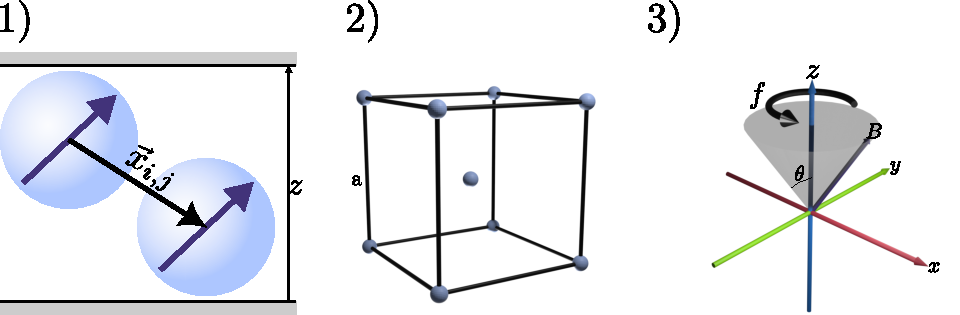
\includegraphics[width=0.95\textwidth]{figures/methods1.pdf}
  \end{center}
  \caption[Representation of the paramagnetic colloids, body-centered-cubic lattice used for the ratchet, and the precessing conic magnetic field.]{\textbf{Panel 1)} Shows two paramagnetic particles with a distance \(\vec{x}_{i,j}\) with the same dipole moment in a confined space in the \( z\) axis. \textbf{Panel 2)} Shows a representation of a  unitary body-centered cubic lattice used in the construction of the ratchet. \textbf{Panel 3} Shows the precessing external magnetic field.}\label{fig:facecenteredlattice}
\end{figure}

Let's remember that one important rule for the universe is that, one body cannot occupy the same space as other, therefore, we should model a repulsion force that simulates that behavior. Fortunately, there is a potential called Weeks-Chandler-Andersen potential (WCA) that follow the same principle as the Lennard-Jones potential but with a cuttof \cite{hess1999augmented}:

\begin{equation}
  U_{i,j}^{WCA} = \begin{cases} 
    4\epsilon\left[ \left( \frac{\sigma}{r_{i,j}}\right)^{12} - \left( \frac{\sigma}{r_{i,j}}\right)^6\right] + \epsilon \quad &r_{i,j} \leq r_c \\
    0 \quad & r_{i,j} \geq r_c
  \end{cases}
  \label{eq:wcapotential}
\end{equation}

where $\sigma$ is the van der Waals radio, it is the point where the energy between the two particles is zero, $\epsilon$ is the well depth, since WCA does not have an attraction interaction, a correction factor of $\epsilon$ is added, and $r_c = 2^{1/6}\sigma$. This however, gives us the enegy between particles, and we need the force, then we apply:

\begin{equation}
 F = - \nabla U, 
  \label{eq:negativegradient}
\end{equation}

getting then

\begin{equation}
  F_{i,j}^{WCA} = \begin{cases} 
    48\epsilon\left[ \left( \frac{\sigma}{r_{i,j}}\right)^{12} - 0.5\left( \frac{\sigma}{r_{i,j}}\right)^6\right]\left[ \frac{1}{r_{i,j}}\right] \quad &r_{i,j} \leq r_c \\
    0 \quad & r_{i,j} \geq r_c
  \end{cases}.
  \label{eq:wcaforce}
\end{equation}

and verifying the interaction between each particle, we obtain:

\begin{equation}
  F^{collision}_i = \sum^{n}_{i \neq j} F^{WCA}_{i,j}.  
  \label{eq:wcasum}
\end{equation}

We want to see how the positions of the particles evolve over time with certain initial conditions, and this equations only compare velocities, this is why we need an integration method.

\section{Velocity Verlet}
%%%%%%%%

The Velocity Verlet algorithm is derived from the standard Verlet method by explicitly incorporating velocity terms \cite{verlet1967computer, chambliss2020magnetic}. We begin with the Taylor series expansions of position.

\subsection{Taylor Series Expansions}

The forward Taylor expansion for position is:
\begin{equation}
    x(t+\Delta t) = x(t) + v(t)\Delta t + \frac{1}{2}a(t)\Delta t^2 + \frac{1}{6}b(t)\Delta t^3 + O(\Delta t^4)
    \label{eq:taylor_forward}
\end{equation}

The backward Taylor expansion is:
\begin{equation}
    x(t-\Delta t) = x(t) - v(t)\Delta t + \frac{1}{2}a(t)\Delta t^2 - \frac{1}{6}b(t)\Delta t^3 + O(\Delta t^4)
    \label{eq:taylor_backward}
\end{equation}
where $b(t)$ represents the third derivative (jerk), and $O(\Delta t^4)$ represents an error of magnitude $\Delta t^4$.

\subsection{Original Verlet Algorithm}

Adding equations (\ref{eq:taylor_forward}) and (\ref{eq:taylor_backward}) cancels the velocity and jerk terms:
\begin{equation}
    x(t+\Delta t) + x(t-\Delta t) = 2x(t) + a(t)\Delta t^2 + O(\Delta t^4)
\end{equation}

Solving for $x(t+\Delta t)$ gives the original Verlet algorithm:
\begin{equation}
    x(t+\Delta t) = 2x(t) - x(t-\Delta t) + a(t)\Delta t^2 + O(\Delta t^4)
    \label{eq:verlet_original}
\end{equation}

\subsection{Velocity Calculation}

Subtracting equation (\ref{eq:taylor_backward}) from (\ref{eq:taylor_forward}) gives the velocity:
\begin{equation}
    x(t+\Delta t) - x(t-\Delta t) = 2v(t)\Delta t + O(\Delta t^3)
\end{equation}
\begin{equation}
    v(t) = \frac{x(t+\Delta t) - x(t-\Delta t)}{2\Delta t} + O(\Delta t^2)
    \label{eq:verlet_velocity}
\end{equation}

\subsection{Velocity Verlet Formulation}

The Velocity Verlet algorithm provides a more convenient form that explicitly tracks velocities. Starting from the forward Taylor expansion (equation \ref{eq:taylor_forward}):
\begin{equation}
    x(t+\Delta t) = x(t) + v(t)\Delta t + \frac{1}{2}a(t)\Delta t^2
    \label{eq:vv_position}
\end{equation}

To find the velocity at $t+\Delta t$, we use the average acceleration:
\begin{equation}
    v(t+\Delta t) = v(t) + \frac{a(t) + a(t+\Delta t)}{2}\Delta t
    \label{eq:vv_velocity_simple}
\end{equation}

A more numerically stable implementation uses a half-step approach:
\begin{align}
    v(t+\tfrac{1}{2}\Delta t) &= v(t) + \frac{1}{2}a(t)\Delta t \\
    a(t+\Delta t) &= \frac{F(x(t+\Delta t))}{m} \quad \text{(Compute new acceleration)} \\
    v(t+\Delta t) &= v(t+\tfrac{1}{2}\Delta t) + \frac{1}{2}a(t+\Delta t)\Delta t
    \label{eq:vv_velocity_halfstep}
\end{align}

\section{Basis Vectors}

The basis vectors (or lattice vectors) are the fundamental building blocks used to generate the entire crystal lattice by translation. These vectors define the geometry of the unit cell, and by repeating the unit cell across space, you form the overall lattice structure. Here, a body-centered latticed was chosen since the stability it prooved to have when under thermal fluctuations.

In the body-centered lattice, the basis vectors determine the relative positions of atoms in the unit cell. These vectors are used to place atoms and generate the positions of all atoms in the simulation box.


The conventional unit cell for a BCC lattice is a cube with a lattice point at each corner and one at the body center. The vectors defining this cube are simple, orthogonal, and given by:
%
\begin{equation}
  \vec{a} = a\hat{x}, \quad \vec{b} = a\hat{y}, \quad \vec{c} = a\hat{z}, \quad \vec{d} = \frac{a}{2}\left(  1\hat{x} +  1\hat{y} + 1\hat{z} \right), 
\end{equation}
%
where \( a \) is the lattice constant (the side length of the cube). However, these points must remain fixed, otherwise these would separate from each other dissolving the structure, therefore we add bonds.

There are multiple forms to model the potential energy of a bond, the easiest way is to use the harmonic potential that mimics the behavior of a ideal spring and is modeled after the Hooke's law:

\begin{equation}
  U^{H}_{i,j}(\vec{x}_{i,j}) = \frac{1}{2}K(\vec{x}_{i,j} - \vec{x}_0)^2,
\end{equation}

where K is the energy per squared distance, $\vec{x}_{i,j}$ is the distance between particle \textit{i}, and \textit{j}, and $x_0$ is the equilibrium distance point.

\begin{figure}
  \begin{center}
    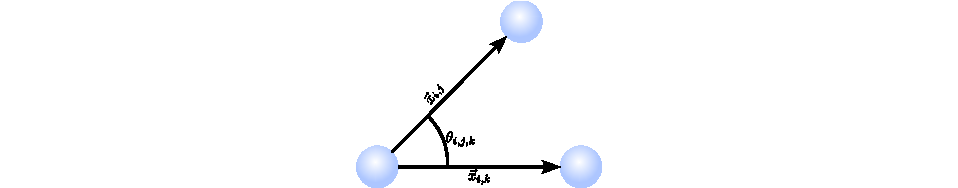
\includegraphics[width=0.95\textwidth]{figures/harmonicP.pdf}
  \end{center}
  \caption[Visual representation for a harmonic potential.]{Visual representation for a harmonic angular potential.}\label{fig:}
\end{figure}


Equally, each particle has a defined angle between a triplet of particles that will help in the definition of the lattice, it is defined also with Hooke's law:

\begin{equation}
  U^{H}_{i,j,k}(\theta _{i,j,k}) = \frac{1}{2}K(\theta_{i,j,k} - \theta_0)^2,
\end{equation}


%%%%%%%%

\section{System Overview and Workflow}

The simulations of this thesis were performed with an open-source software called LAMMPS (Large-scale Atomic/Molecular Massively Parallel Simulator) developed by Sandia National Laboratories. Its advantage is the high efficiency to run simulatios in parallel, reducing the time required to perform multiple calculations \cite{LAMMPS}. We used a standard version of LAMMPS but created custom input scripts using a Python library. These scripts will atomate the process of the input scritpts that will tell LAMMPS everything about the parameters of our simulation, such as the size of the system, the physical conditions, and how long to run for. After the simulations, we used additional custom scripts with the help of a Python library called Pandas, to analyze the results quickly and efficiently.

\begin{figure}[h]
  \begin{center}
    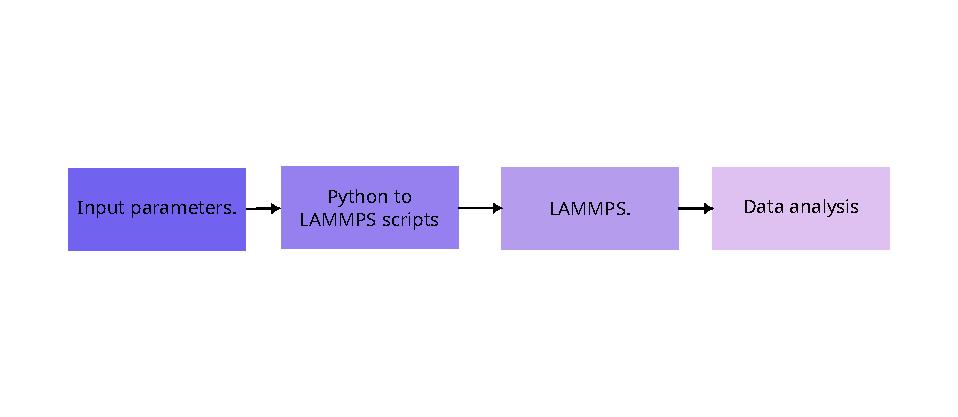
\includegraphics[width=0.95\textwidth]{figures/workflow.pdf}
  \end{center}
  \caption[Workflow diagram.]{Workflow diagram.}\label{fig:workflow}
\end{figure}

\subsection{System's Physical Definition}

The first parameters to be defined are the ones from the circular-ratchet geometry, since it will define the position of the paramagnetic colloids afterwards, these are the parameters that can be specified in the function:

\begin{table}[H]
\centering
\caption[Ratchet physical parameters.]{Parameters used for the circular ratchet in the simulation.}
\begin{tabular}{l l l l l}
\hline
Parameter & Symbol & Ratchet A & Ratchet B & Units \\
\hline
Lattice constant & \(a\) & 1 & 1 & \(\mu m\) \\
Radius & \( r\) & 8 & 8 & \( \mu m\) \\
Sawtooth amplitude & \( A\) & 4 & 4 & \( \mu m\) \\
Sawtooth frequency & \( N\) & 5 & 3 & Dimensionless\\
Bond coefficient & \( K_b\) & 0.1 & 0.1 & \( \mu N\) \\ 
Density & \(\rho\) & 1 & 1 & kgm\(^{-3}\) \\
\hline
\end{tabular}
\end{table}

\begin{figure}
  \begin{center}
    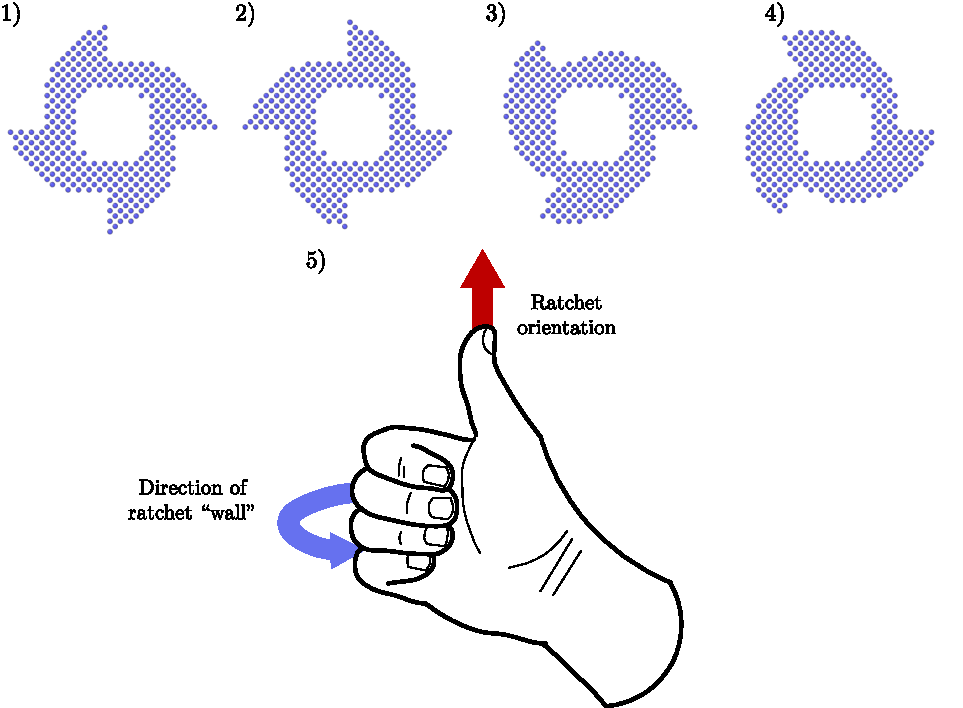
\includegraphics[width=0.95\textwidth]{figures/ratchet.pdf}
  \end{center}
  \caption[Ratchet geomety.]{Ratchet geometry used in the simulations. \textbf{Panel 1)} shows 4-spikes ratchet.\textbf{Panel 2)} shows the same ratchet with a 180° specular rotation. \textbf{Panel 3) - 4)} Shows the same characterisitcs with a 3-spikes ratchet. \textbf{ Panel 5)} Shows the convention used for classifying the ratchets. In this case the curl right hand rule can be used. Facing the ``wall'' of the ratchet with the palm of the hand, the thumb will indicate the geometry of the ratchet. If the thumb points towards you or upwards, the geometry will be called spin up, if it points downwards the geometry will be called spin down.}\label{fig:ratchetgeometry}
\end{figure}


As shown in the previous table, there were 2 ratchets with only a difference in te \textit{Sawtooth frequency}, but in reality we used a reflection of each ratchet for another pair of analysis. Once the ratchet geometry is defined, then we can define then the remaining of the system, which remained constant for the 2 ratchets. Starting with the simulation box, that is a rectangle box of periodic boundary conditions in axis \textit{x}, and \textit{y},and finite boundary conditions modeled with the a WCA potential:



\begin{table}[H]
\centering
\caption[Simulation box physical parameters.]{Parameters used for the box of the simulation.}
\begin{tabular}{l l l l}
\hline
Axis & lo  & hi & Units \\
\hline
\textit{x} & -27 & 27 & \( \mu m\) \\
\textit{y} & -27 & 27 & \( \mu m\) \\
\textit{z} & -2  & 2   & \( \mu m\)\\ 
\hline
\end{tabular}
\end{table}

Where \textit{lo} represent the lower boundary, an \textit{hi} the upper boundary.

Finally, for the paramagnetic particles, and since they deppend on the magnetci field, we included the parameters of this one too


\begin{table}[H]
\centering
\caption[Paramagnetic colloids parameters.]{Parameters used for the paramagnetic particles.}
\begin{tabular}{l l l l}
\hline
Parameter & Symbol  & Value & Units \\
\hline
Radius & $r_{mag}$ &  1.25 &\( \mu m\) \\
Susceptibility & $\chi$ & 0.4 & Dimensionless\\
Field angle & $\theta$ & 27 & °\\
Frequency & $f$ & [0 - 10] & Hz\\
\hline
\end{tabular}
\end{table}

With all this values, we can run simulations for a period of $50 \cross 10^6$ frames, with a timestep of 10 $\mu s$ which corresponds to a total real time of $500 s$ ($8.33\bar{3} \mathrm{min})$. Since these systems are of random nature, it is recommended to perform multiple simulations in order to be able to obtain statistics, therefore we ran it 10 different times for each frequency.

\subsection{Data Analysis}

When finishing a simulation, LAMMPS will give a text data file with values we chose to obtain. In this case we were interesented in the position of the particles to be able to deduce some information, being the angular velocity the more interesting one. The system consist of multiple particles, each one of them having a different angular velocity due to bond not being strong enough to mantain particles static, therefore we need to obtain an average velocity for the entirety of the particles. What we know, is that every particle shares the same center of mass that is calculated as follows:

\begin{equation}
  (x_{\mathrm{COM}}, y_{\mathrm{COM}}) = \displaystyle\frac{\sum^{n}_{i=1} m_i * r_i}{\sum^{n}_{i=1} m_i}.
  \label{eq:centerofmass}
\end{equation}

Being $m_i$ the mass of the particle \textit{i}, and $r_i$ the position of the particle respect a frame of reference. The best way to calculate the angular velocity is by using polar coordinates:

\begin{align}
  r_i & = \sqrt{(x - x_{\mathrm{COM}})^2 + (y - y_{\mathrm{COM}})^2},\\ 
  \theta _i &= \arctan{\frac{y - y_{\mathrm{COM}}}{x - x_{\mathrm{COM}}}}.
\end{align}

Once obtained the center of mass and the polar coordinates of each particle, then we can calculate the angular velocity of each particle for each timestep of the simulation:
\begin{equation}
  \omega _i = \frac{\Delta \theta _i}{\Delta t},
  \label{eq:angularvelocity}
\end{equation}

then obtaining an average angular velocity of all particles.

